\documentclass{report}

\usepackage{mathtools, amsthm, amsmath, amssymb}
\usepackage{babel}
\usepackage[thaifont=TH Sarabun New]{thaispec}
\usepackage{biblatex}
\addbibresource{db.bib}

\title{ฐานข้อมูล\\ร้านขายคุกกี้}
\author{    
\begin{tabular}{ll}
	นางสาวอนาตี มะหะหมัด 116510901022-3\\นางสาวศุภศรี คงชื่นจิตร 116510901023-1\\นางสาวอริศรา ธนทรัพย์ไพรฑูรย์ 116510901024-9
\end{tabular}\\ 
\\
เสนอ\\
ดร.รัฐพรหม พรหมคำ\\
รองศาสตราจารย์ ดร.วงศ์วิศรุต เขื่องสตุ่ง\\
\\
สาขาวิชาคณิตศาสตร์ คณะวิทยาศาสตร์และเทคโนโลยี\\
มหาวิทยาลัยเทคโนโลยีราชมงคลธัญบุรี
}
\date{2 พฤศจิกายน 2567}

\begin{document}
\maketitle
\tableofcontents
\listoffigures

\pagebreak

\begin{center}
\textbf{บทคัดย่อ } 
\end{center}
การพัฒนาฐานข้อมูลสําหรับร้านคุกกี้มีวัตถุประสงค์เพื่อจัดการข้อมูลสินค้าคุกกี้, ลูกค้า, และการสั่งซื้ออย่างมีประสิทธิภาพ ระบบฐานข้อมูลนี้ถูกออกแบบมาเพื่อตอบสนองความต้องการในการเก็บข้อมูลที่มีความหลากหลาย รวมถึงชื่อคุกกี้, ราคา, ส่วนผสม, และปริมาณสต็อก นอกจากนี้ยังมีการจัดเก็บข้อมูลลูกค้าเพื่อช่วยในการวิเคราะห์พฤติกรรมการซื้อและสร้างความสัมพันธ์ที่ดีกับลูกค้า การใช้ฐานข้อมูลเชิงสัมพันธ์ทําให้สามารถดึงข้อมูลที่ต้องการได้อย่างรวดเร็วและแม่นยําการวิจัยนี้ยังได้สํารวจเทคโนโลยีต่าง ๆ ที่สามารถนำมาใช้ในการพัฒนาระบบ เช่น SQL และโปรแกรมจัดการฐานข้อมูล เพื่อให้สามารถจัดการข้อมูลได้อย่างมีประสิทธิภาพ ผลลัพธ์ที่ได้จากการพัฒนาฐานข้อมูลนี้จะช่วยเพิ่มประสิทธิภาพในการดําเนินงานของร้านคุกกี้ และยกระดับประสบการณ์ของลูกค้าในกระบวนการสั่งซื้อ

\begin{center}
\chapter{บทนำ}
\end{center}
\section{ที่มาและความสำคัญ}
โครงงานฉบับนี้ได้จัดทําขึ้นเพื่อประโยชน์สําหรับศึกษาและเรียนรู้ในการสร้างระบบฐานข้อมูลที่มีประสิทธิภาพของร้านคุกกี้ \par

ในปัจจุบัน ตลาดขนมอบและคุกกี้มีการเติบโตอย่างรวดเร็ว โดยเฉพาะอย่างยิ่งในยุคดิจิทัลที่ผู้บริโภคมีแนวโน้มที่จะเลือกซื้อสินค้าออนไลน์มากขึ้น ร้านคุกกี้จึงจําเป็นต้องปรับตัวเพื่อให้สามารถตอบสนองความต้องการของลูกค้าได้อย่างมีประสิทธิภาพ การจัดการข้อมูลเกี่ยวกับสินค้าคุกกี้, ลูกค้า, และการสั่งซื้อจึงเป็นปัจจัยที่สําคัญที่จะช่วยให้ร้านค้าสามารถดําเนินงานได้อย่างราบรื่น

การที่ร้านคุกกี้ไม่มีระบบฐานข้อมูลที่มีประสิทธิภาพอาจนําไปสู่ปัญหาหลายประการ เช่น ข้อมูลสินค้าที่ไม่เป็นปัจจุบัน,ความยุ่งเหยิงในการจัดการคำสั่งซื้อ, และความล่าช้าในการให้บริการลูกค้า นอกจากนี้ ข้อมูลที่ถูกจัดเก็บในลักษณะที่ไม่มีระบบอาจทําให้การวิเคราะห์พฤติกรรมการซื้อของลูกค้าเป็นไปได้ยาก ส่งผลให้ร้านค้าขาดข้อมูลที่จําป็นในการพัฒนากลยุทธ์การตลาดและการสร้างความสัมพันธ์ที่ดีกับลูกค้า
การพัฒนาฐานข้อมูลสำหรับร้านคุกกี้จึงมีความสำคัญอย่างยิ่ง เพราะจะช่วยให้การจัดการข้อมูลเป็นไปอย่างมีระเบียบ สามารถเข้าถึงข้อมูลได้อย่างรวดเร็วและแม่นยํารวมถึงสามารถสร้างรายงานการขายและการวิเคราะห์ข้อมูลต่าง ๆ ได้อย่างมีประสิทธิภาพ นอกจากนี้ ฐานข้อมูลที่ดีจะช่วยให้ร้านค้าสามารถติดตามแนวโน้มการตลาดและปรับตัวให้เข้ากับความต้องการของลูกค้าได้ทันท่วงทีด้วยเหตุนี้ การสร้างฐานข้อมูลที่มีโครงสร้างและการจัดการที่เหมาะสมจึงเป็นสิ่งจําป็นเพื่อเสริมสร้างความสามารถในการแข่งขันของร้านคุกกี้ และช่วยให้สามารถเติบโตอย่างยั่งยืนในตลาดที่มีการแข่งขันสูง\par

ดังนั้นคณะผู้จัดทําหวังเป็นอย่างยิ่งว่าระบบฐานข้อมูลเล่มนี้ได้รวบรวมเนื้อหาที่เป็นประโยชน์แก่ผู้สนใจ และทําความเข้าใจลักษณะของการสร้างระบบฐานข้อมูลรวมไปถึงการสร้างความน่าสนใจในตลาดตลอดจนทําการศึกษาเพิ่มเติม เพื่อนำไปจัดทำต่อยอดได้ในเชิงธุรกิจ ที่มีความเหมาะสมในเชิงปฏิบัติมากขึ้น

\section{วัตถุประสงค์}
\begin{itemize} 
	\item สร้างระบบฐานข้อมูลที่มีประสิทธิภาพ
	\item เพิ่มประสิทธิภาพในการจัดการข้อมูล
	\item สนับสนุนการวิเคราะห์ข้อมูล
	\item พัฒนาประสบการณ์ของลูกค้า
	\item ส่งเสริมการเติบโตของธุรกิจ
\end{itemize}
\section{ประโยชน์ที่คาดว่าจะได้รับ}
\begin{itemize}
    \item จัดการข้อมูลได้มีประสิทธิภาพ
    \item เพิ่มความรวดเร็วในการดำเนินงาน
    \item เข้าใจพฤติกรรมลูกค้าได้ดีขึ้น
    \item ปรับปรุงบริการลูกค้า
    \item เพิ่มยอดขาย
\end{itemize}
\section{ขอบเขต}
\begin{itemize}
    \item{ระบบจะจัดเก็บและจัดการข้อมูลสินค้า คำสั่งซื้อ และสต็อค พร้อมฟังก์ชันการเข้าถึงและวิเคราะห์ข้อมูลเพื่อสนับสนุนการดํานินงานของร้านคุกกี้ }
\end{itemize}

\chapter{ความรู้ทั่วไป}
\section{ซอฟคุกกี้}
\begin{figure}[h!]
	\centering
	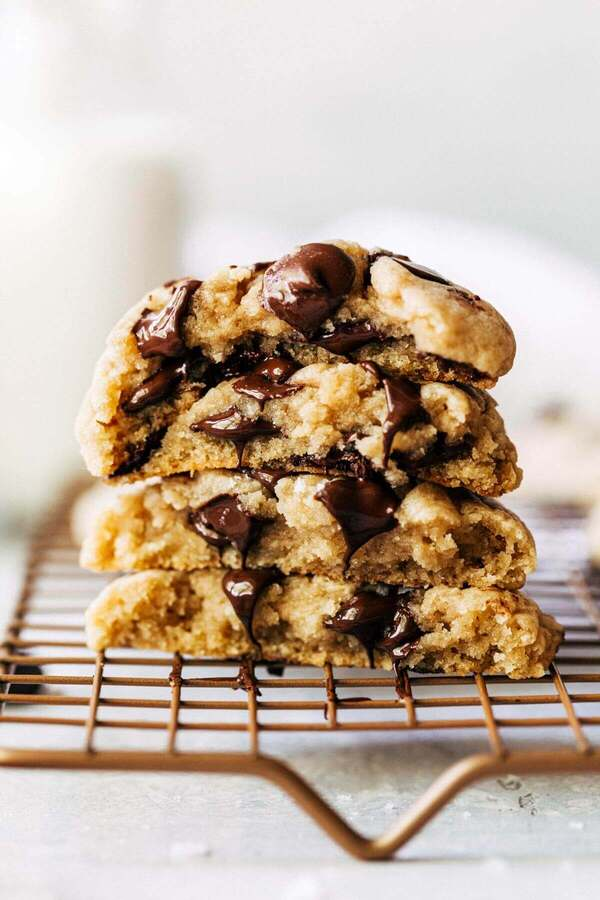
\includegraphics[scale=0.25]{aa.jpg}
	\caption{ภาพซอฟคุกกี้ \cite{YOYO}}
	\label{fig:graph1} 
\end{figure}
ซอฟคุกกี้ (Soft Cookies) เป็นคุกกี้ที่มีเนื้อสัมผัสนุ่มและชุ่มชื้น มักจะมีรสชาติหวานและกรอบบางส่วน แต่โดยรวมจะนุ่มและละลายในปาก ในการทำซอฟคุกกี้ ส่วนผสมและเทคนิคจะมีความสำคัญมาก เพื่อให้ได้ผลลัพธ์ที่นุ่มและอร่อย
\textbf{ประวัติของซอฟคุกกี้}  \par 
ซอฟคุกกี้มีประวัติที่น่าสนใจ ซึ่งเกี่ยวข้องกับการพัฒนาของคุกกี้โดยรวม ตั้งแต่ต้นกำเนิดของคุกกี้ในยุโรปจนถึงการแพร่หลายไปทั่วโลกในสมัยปัจจุบัน
\section{ต้นกำเนิด}	\par
\begin{itemize} 
	\item ยุคกลาง คุกกี้เริ่มมีการทำขึ้นในยุโรปตั้งแต่ยุคกลาง โดยใช้ส่วนผสมง่ายๆ เช่น แป้ง น้ำตาล และไข่ เพื่อสร้างขนมอบที่สามารถเก็บได้นาน
	\item ศตวรรษที่ 17 ในศตวรรษนี้ คุกกี้เริ่มถูกทําให้หลากหลายขึ้นโดยเฉพาะในประเทศเนเธอร์แลนด์และอังกฤษ ซึ่งเริ่มมีการเพิ่มส่วนผสมต่างๆ เช่น เครื่องเทศและผลไม้แห้ง
\end{itemize}
\section{การพัฒนาซอฟคุกกี้}	\par
\begin{itemize}
	\item คุกกี้ช็อกโกแลตชิป ในปี 1938 Ruth Wakefield เจ้าของโรงแรม Toll House ในรัฐแมสซาชูเซตส์ ได้สร้างคุกกี้ช็อกโกแลตชิป โดยการเพิ่มช็อกโกแลตชิปลงในสูตรคุกกี้น้ำตาล นี่ถือเป็นจุดเริ่มต้นของซอฟคุกกี้ในรูปแบบที่เรารู้จักกันในปัจจุบัน
	\item ความนิยม คุกกี้ช็อกโกแลตชิปได้รับความนิยมอย่างรวดเร็ว และซอฟคุกกี้ก็เริ่มมีการทำและพัฒนาในหลากหลายสูตรและรูปแบบในทั่วทั้งสหรัฐอเมริกา
\end{itemize}
\section{การแพร่หลายทั่วโลก} \par
\begin{itemize}
	\item สหรัฐอเมริกาซอฟคุกกี้กลายเป็นขนมที่ได้รับความนิยมในหลายโอกาส ไม่ว่าจะเป็นการทำที่บ้านหรือการขายในร้านขนม
	\item วัฒนธรรมอื่น ซอฟคุกกี้ยังมีการดัดแปลงในหลายวัฒนธรรม โดยอาจมีการเพิ่มส่วนผสมที่เป็นเอกลักษณ์ เช่น การใช้ชาเขียวในญี่ปุ่นหรือการเติมกลิ่นหอมของมะพร้าวในเอเชียตะวันออกเฉียงใต้
\end{itemize}
\section{ลักษณะของซอฟคุกกี้} \par
\begin{itemize}
	\item เนื้อสัมผัส ซอฟคุกกี้มีความนุ่มและบางครั้งอาจจะมีเนื้อกรอบที่ขอบ แต่โดยรวมแล้วจะมีความชุ่มชื้น
	\item รสชาติ มักจะมีรสชาติหวาน มีการใช้ส่วนผสมเสริมอย่างช็อกโกแลตชิป ถั่ว หรือผลไม้อบแห้งเพื่อเพิ่มความหลากหลาย
\end{itemize}
\section{ส่วนผสมหลัก} \par
\begin{enumerate}
	\item เนย ให้ความชุ่มชื้นและรสชาติอร่อย
	\item น้ำตาล มักใช้ทั้งน้ำตาลทรายและน้ำตาลไอซิ่ง
	\item ไข่ ช่วยในการยึดเนื้อและทำให้คุกกี้มีความนุ่ม
	\item แป้ง แป้งสาลีเป็นส่วนผสมหลัก
	\item เบกกิ้งโซดา ช่วยให้คุกกี้ฟูขึ้น
\end{enumerate}
\section{วิธีการทำ} \par
\begin{enumerate}
	\item ตีเนยและน้ำตาล: จนเข้ากันดีและฟู
	\item เติมไข่: แล้วตีให้เข้ากัน
	\item ผสมแห้ง: แป้ง เบกกิ้งโซดา และเกลือผสมกันแล้วนำไปใส่ในส่วนผสมเปียก
	\item เพิ่มวัตถุดิบเสริม: เช่น ช็อกโกแลตชิป หรือถั่ว
	\item อบ: อบที่อุณหภูมิประมาณ 170-180 องศาเซลเซียส จนเริ่มมีสีทองที่ขอบ แต่ยังนุ่มอยู่ตรงกลาง
\end{enumerate}

\chapter{ปัญหาและการแก้ปัญหาจากฐานข้อมูลที่สร้างขึ้น}

\section{ฐานข้อมูล}
\begin{figure}[!ht]
	\centering
	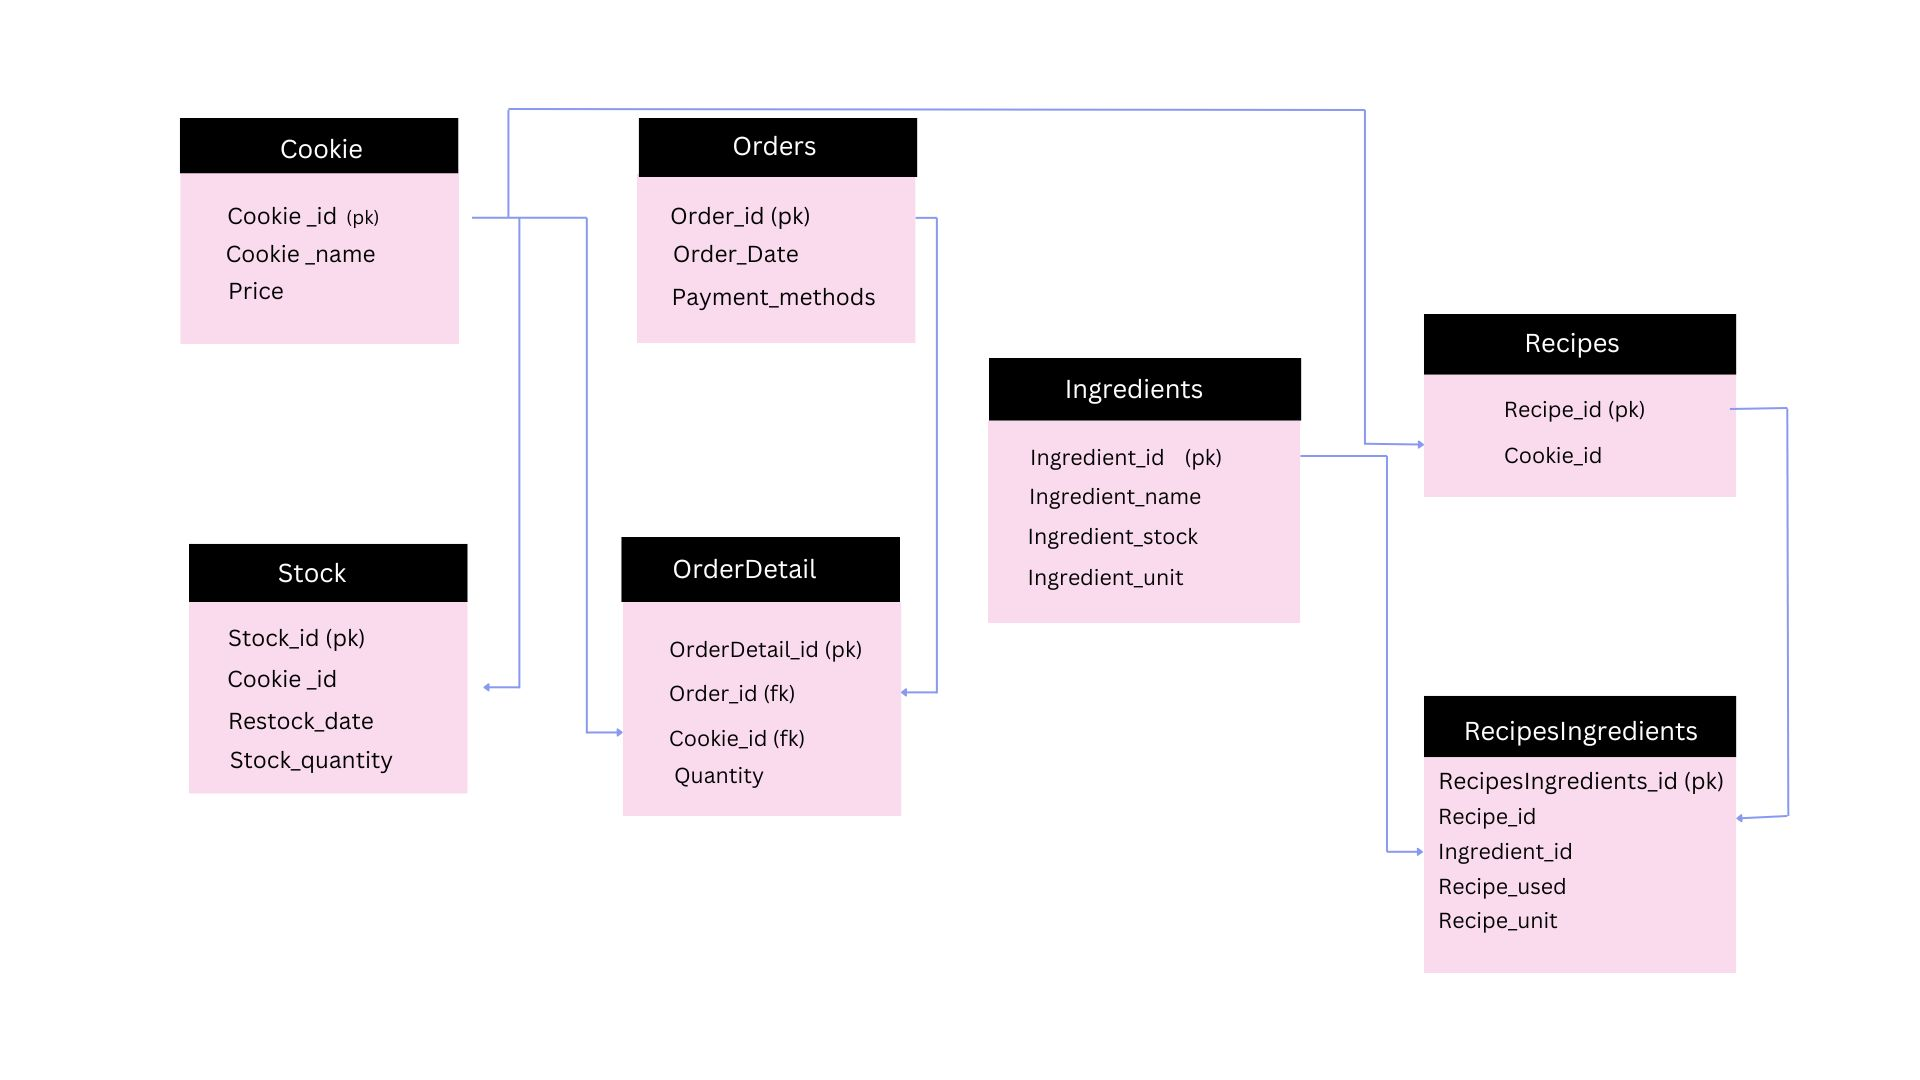
\includegraphics[scale=0.3]{Menu.jpg}
	\caption{แผนภาพ diagram}
	\label{fig : graph2}
\end{figure}

\section{ปัญหา}
\begin{enumerate}
	\item เบเกอรี่ชนิดไหนที่ขายออกได้น้อยที่สุด
	\item วัตถุดิบแต่ละสต็อคใช้ออกไม่หมด
	\item ช่วงเวลาที่มียอดขายมากที่สุด
	\item ช่องทางการชำระเงินที่ลูกค้านิยมมากที่สุด
\end{enumerate}

\section{codeที่ใช้ตอบปัญหา}

\textbf{ปัญหาที่1} 
\begin{verbatim}
SELECT
	 cookie_id,
	 SUM(Quantity) AS Quantity
FROM Orders 
WHERE cookie_id
GROUP BY cookie_id
ORDER BY Quantity ASC
LIMIT 1;  
\end{verbatim}
\textbf{ผลลัพธ์}
\raggedright\begin{figure}[!ht]
    \centering
    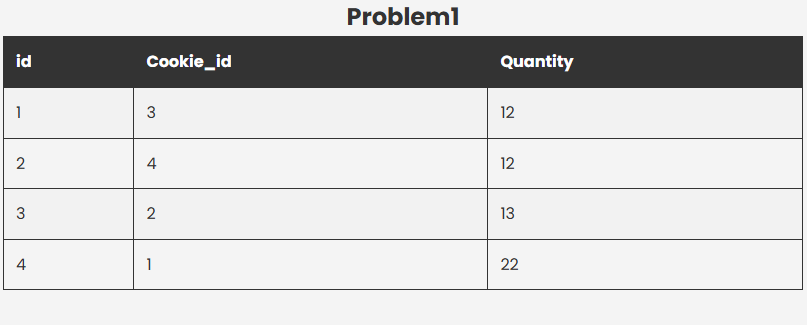
\includegraphics[scale=0.55]{q1.png}
    \caption{ผลลัพธ์จากโค้ดข้างต้น} 
\label{fig:mesh1}
\end{figure} 


\pagebreak\textbf{ปัญหาที่2} 
\begin{verbatim}
SELECT i.Ingredients_name, i.Ingredients_stock,
 
       COALESCE(SUM(r.Recipes_used), 0) AS total_used,
	   i.ingredients_unit
 
FROM Ingredients AS i
 
LEFT JOIN Recipes AS r ON i.ingredients_id = r.Ingredients_id
 
GROUP BY i.Ingredients_name, i.Ingredients_stock
 
HAVING i.Ingredients_stock - COALESCE(SUM(r.Recipes_used), 0) > 0
 
ORDER BY i.Ingredients_stock ASC;
\end{verbatim}
\textbf{ผลลัพธ์}
\raggedright\begin{figure}[!ht]
    \centering
    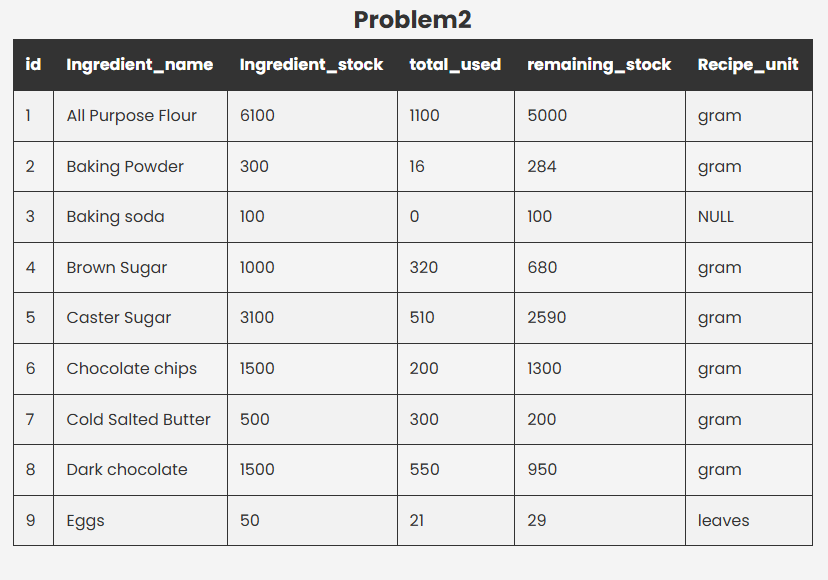
\includegraphics[scale=0.55]{q2.png}
    \caption{ผลลัพธ์จากโค้ดข้างต้น} 
\label{fig:mesh2}
\end{figure} 


\par
\pagebreak\textbf{ปัญหาที่3} 
\begin{verbatim}
SELECT
    Order_Date,
    COUNT(*) AS Total_orders
FROM Orders
GROUP BY Order_Date
ORDER BY Total_orders DESC
LIMIT 1;
\end{verbatim}
\textbf{ผลลัพธ์}
\raggedright\begin{figure}[!ht]
    \centering
    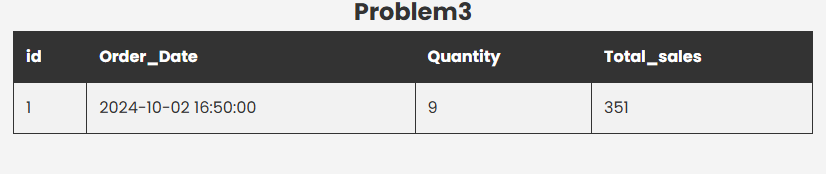
\includegraphics[scale=0.55]{q3.png}
    \caption{ผลลัพธ์จากโค้ดข้างต้น} 
\label{fig:mesh2}
\end{figure}



\par
\textbf{ปัญหาที่4} 
\begin{verbatim}
SELECT
	Payment_methods,
	COUNT(*) AS Total_payment
FROM Orders 
GROUP BY Payment_methods
ORDER BY Total_payment DESC
LIMIT 1;
\end{verbatim}
\textbf{ผลลัพธ์}
\raggedright\begin{figure}[!ht]
    \centering
    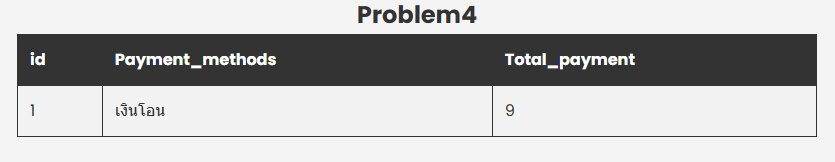
\includegraphics[scale=0.55]{q4.png}
    \caption{ผลลัพธ์จากโค้ดข้างต้น} 
\label{fig:mesh2}
\end{figure}

\chapter{การสร้างหน้าเว็บเพจร้านคุกกี้ (Cookie shop)}

\section{โค้ด index.htmlและ style.css}
\textbf{index}
\begin{verbatim}
<!DOCTYPE html>
<html lang="en">
<head>
<meta charset="UTF-8">
<meta name="viewport" content="width=device-width, initial-scale=1.0">
<title>Cookie Shop</title>
<link rel="stylesheet" href="styles.css">
<link rel="preconnect" href="https://fonts.gstatic.com">
<link href="https://fonts.googleapis.com/css2?family=Poppins:wght@400;600;700&display=swap" rel="stylesheet">
<link rel="stylesheet" type="text/css" href="https://cdnjs.cloudflare.com/ajax/libs/font-awesome/6.6.0/css/all.min.css">
</head>
<body>
<header class="header">
<div class="container">
<div class="header__logo">Cookie Shop</div>
<nav class="header__nav">
<ul>
<li><a href="#">Home</a></li>
<li><a href="menu.html">Menu</a></li>
<li><a href="about.html">About</a></li>
<li><a href="contact.html">Contact</a></li>
<li><a href="html.html"><i class="fas fa-magnifying-glass"></i></a></li>
</ul>
</nav>
</div>
</header>
 
  <main>
<section class="hero">
<div class="container">
<video src="coki.mp4" muted loop autoplay></video>
<h1 class="hero__title">Soft Cookie</h1>
<p class="hero__description">Indulge in our homemade, artisanal cookies</p>
<a href="menu.html" class="hero__cta">Explore Menu</a>
</div>
</section>
<div class="page-wrapper">
<!-- Header Section -->
<div class="showcase-header">
<h2 class="main-title">History of Cookies</h2>
<p class="intro-text">Cookies are a snack that can be stored for a long time. This is an advantage that makes tourists or people who like to travel often have them with them. Whenever you are hungry, you can take them out and eat them at any time because they have a long shelf life and do not spoil easily.</p>
<p class="intro-text">Cookies are snacks that are kept at home as a snack while drinking tea or coffee. There are many types, up to 6 types, consisting of drop cookies, roll cookies, pressed cookies, molded cookies, bar cookies or bar cookies.</p>
</div>
 
    <div class="showcase-section">
<h3 class="section-title">Types of Cookies</h3>
<div class="gallery-grid">
<!-- Dropped Cookies -->
<div class="product-card">
<img src="dro.jpg" alt="Dropped Cookies" class="product-image">
<div class="product-info">
<h4 class="product-name">Dropped Cookies</h4>
</div>
</div>
 
                <!-- Rolled Cookies -->
<div class="product-card">
<img src="ro.jpg" alt="Rolled Cookies" class="product-image">
<div class="product-info">
<h4 class="product-name">Rolled Cookies</h4>
</div>
</div>
 
                <!-- Pressed Cookies -->
<div class="product-card">
<img src="m.jpg" alt="Pressed Cookies" class="product-image">
<div class="product-info">
<h4 class="product-name">Pressed Cookies</h4>
</div>
</div>
 
                <!-- Moulded Cookies -->
<div class="product-card">
<img src="p.jpg" alt="Moulded Cookies" class="product-image">
<div class="product-info">
<h4 class="product-name">Moulded Cookies</h4>
</div>
</div>
 
                <!-- Bar Cookies -->
<div class="product-card">
<img src="b.jpeg" alt="Bar Cookies" class="product-image">
<div class="product-info">
<h4 class="product-name">Bar Cookies</h4>
</div>
</div>
 
                <!-- Refrigerated Cookies -->
<div class="product-card">
<img src="r.jpg" alt="Refrigerated Cookies" class="product-image">
<div class="product-info">
<h4 class="product-name">Refrigerated Cookies</h4>
</div>
</div>
</div>
</div>
</div>
 
    </section>  
<section class="features">
<div class="container">
<h2 class="features__title">Why Choose Our Cookies?</h2>
<div class="features__grid">
<div class="feature">
<i class="fas fa-cookie-bite"></i>
<h3>Freshly Baked</h3>
<p>Baked fresh daily using premium ingredients</p>
</div>
<div class="feature">
<i class="fas fa-award"></i>
<h3>Quality Guaranteed</h3>
<p>100% satisfaction guaranteed or your money back</p>
</div>
<div class="feature">
<i class="fas fa-truck"></i>
<h3>Fast Delivery</h3>
<p>Same day delivery available</p>
</div>
</div>
</div>
</section>
 
    <section class="reviews">
<div class="container">
<h2 class="reviews__title">What Our Customers Say</h2>
<div class="reviews__grid">
<div class="review-card">
<div class="review-card__profile">
<img src="n.jpg" alt="Customer" class="review-card__image">
<div class="review-card__info">
<h3>Sarah Johnson</h3>
<div class="review-card__stars">
<i class="fas fa-star"></i>
<i class="fas fa-star"></i>
<i class="fas fa-star"></i>
<i class="fas fa-star"></i>
<i class="fas fa-star"></i>
</div>
</div>
</div>
<p class="review-card__text">"The chocolate chip cookies are absolutely divine! Crispy on the outside, soft on the inside - perfect with my morning coffee."</p>
<span class="review-card__date">2 days ago</span>
</div>
 
      <div class="review-card">
<div class="review-card__profile">
<img src="k.jpg" alt="Customer" class="review-card__image">
<div class="review-card__info">
<h3>Mike Chen</h3>
<div class="review-card__stars">
<i class="fas fa-star"></i>
<i class="fas fa-star"></i>
<i class="fas fa-star"></i>
<i class="fas fa-star"></i>
<i class="fas fa-star-half-alt"></i>
</div>
</div>
</div>
<p class="review-card__text">"Best cookie shop in town! The oatmeal raisin cookies remind me of my grandmother's recipe. Will definitely be back for more!"</p>
<span class="review-card__date">1 week ago</span>
</div>
 
      <div class="review-card">
<div class="review-card__profile">
<img src="o.jpg" alt="Customer" class="review-card__image">
<div class="review-card__info">
<h3>Emma Davis</h3>
<div class="review-card__stars">
<i class="fas fa-star"></i>
<i class="fas fa-star"></i>
<i class="fas fa-star"></i>
<i class="fas fa-star"></i>
<i class="fas fa-star"></i>
</div>
</div>
</div>
<p class="review-card__text">"The variety is amazing! Tried the macadamia white chocolate cookies and they were heavenly. Great customer service too!"</p>
<span class="review-card__date">3 days ago</span>
</div>
</div>
<div class="review-form">
<h3 class="review-form__title">Share Your Experience</h3>
<form class="review-form__container">
<div class="review-form__rating">
<span>Your Rating:</span>
<div class="star-rating">
<i class="far fa-star"></i>
<i class="far fa-star"></i>
<i class="far fa-star"></i>
<i class="far fa-star"></i>
<i class="far fa-star"></i>
</div>
</div>
<textarea placeholder="Write your review here..." required></textarea>
<button type="submit">Submit Review</button>
</form>
</div>
</div>
</section>
</body>
</html>
\end{verbatim}
\textbf{css}
\begin{verbatim}
* {
  margin: 0;
  padding: 0;
  box-sizing: border-box;
  font-family: 'Poppins', sans-serif;
}
 
body {
  line-height: 1.6;
  color: #333;
}
 
.container {
  max-width: 1200px;
  margin: 0 auto;
  padding: 0 20px;
}
 
/* Header Styles */
.header {
  position: fixed;
  top: 0;
  left: 0;
  right: 0;
  background: #fff;
  box-shadow: 0 2px 5px rgba(0,0,0,0.1);
  z-index: 1000;
}
 
.header .container {
  display: flex;
  justify-content: space-between;
  align-items: center;
  height: 80px;
}
 
.header__logo {
  font-size: 1.5rem;
  font-weight: 600;
}
 
.header__nav ul {
  display: flex;
  list-style: none;
  gap: 2rem;
}
 
.header__nav a {
  text-decoration: none;
  color: #333;
  font-weight: 500;
  transition: color 0.3s;
}
 
.header__nav a:hover {
  color: #666;
}
 
.hero {
  position: relative;
  height: 100vh;
  display: flex;
  align-items: center;
  text-align: left;
  padding: 0 5%;
  color: #fff;
  overflow: hidden; /* ป้องกันวิดีโอที่เกินขอบเขตของ .hero */
}
 
.hero video {
  position: absolute;
  top: 0;
  left: 0;
  width: 100%;
  height: 100%;
  object-fit: cover;
  z-index: -1; /* ให้วิดีโออยู่ด้านหลังเนื้อหา */
  opacity: 0.5; /* ปรับความทึบเพื่อให้เนื้อหาอ่านได้ง่ายขึ้น */
}
 
.hero__title {
  font-size: 4rem;
  font-weight: 700;
  color: #000;
  margin-bottom: 1rem;
}
 
.hero__description {
  font-size: 1.2rem;
  color: #000;
  margin-bottom: 2rem;
 
}
 
.hero__cta {
  display: inline-block;
  padding: 1rem 2rem;
  background: #000;
  color: #fff;
  text-decoration: none;
  border-radius: 4px;
  font-weight: 500;
  transition: background 0.3s;
}
 
.hero__cta:hover {
  background: #f0f0f0;
}
 
.contens{
  display: inline-block;
  padding: 3rem 5rem;
  color: #000;
  text-decoration: none;
  border-radius: 4px;
  font-weight: 500;
  transition: background 0.3s;
}
 
.con-ten{
  font-size: 2rem;
  font-weight: 600;
  justify-content: center;
  margin: 0;
}
 
.con-info{
  font-size: 4rem;
  font-weight: 700;
  color: #000;
  padding:2rem 3rem ;
  margin-bottom: 1rem;
}
 
.type{
  font-size: 4rem;
  display: flex;
  justify-content: center;
  align-items: center;
}
.page-wrapper {
    max-width: 1200px;
    margin: 0 auto;
    padding: 2rem;
}
 
/* Header Section */
.showcase-header {
    text-align: center;
    margin-bottom: 3rem;
}
 
.main-title {
    font-size: 2.5rem;
    color: #333;
    margin-bottom: 1.5rem;
}
 
.intro-text {
    color: #666;
    line-height: 1.6;
    max-width: 800px;
    margin: 0 auto 1rem;
}
 
/* Types Section */
.section-title {
    text-align: center;
    font-size: 2rem;
    color: #333;
    margin-bottom: 2rem;
}
 
.gallery-grid {
    display: grid;
    grid-template-columns: repeat(auto-fit, minmax(300px, 1fr));
    gap: 2rem;
    padding: 1rem;
}
 
.product-card {
    background: white;
    border-radius: 10px;
    overflow: hidden;
    box-shadow: 0 4px 6px rgba(0, 0, 0, 0.1);
    transition: transform 0.3s ease;
}
 
.product-card:hover {
    transform: translateY(-5px);
}
 
.product-image {
    width: 100%;
    height: 200px;
    object-fit: cover;
}
 
.product-info {
    padding: 1.5rem;
    text-align: center;
}
 
.product-name {
    font-size: 1.25rem;
    color: #333;
    margin-bottom: 0.5rem;
}
 
/* Responsive Design */
@media (max-width: 768px) {
    .page-wrapper {
        padding: 1rem;
    }
 
    .main-title {
        font-size: 2rem;
    }
 
    .gallery-grid {
        grid-template-columns: repeat(auto-fit, minmax(250px, 1fr));
        gap: 1rem;
    }
 
    .product-image {
        height: 180px;
    }
}
 
/* About Section */
.about {
  padding: 5rem 0;
  background: #ffff;
  text-align: center;
}
 
.about__title {
  font-size: 2rem;
  margin-bottom: 1rem;
}
 
.about__description {
  max-width: 600px;
  margin: 0 auto 2rem;
}
 
.about__cta {
  display: inline-block;
  padding: 1rem 2rem;
  background: #333;
  color: #fff;
  text-decoration: none;
  border-radius: 4px;
  transition: background 0.3s;
}
 
.about__cta:hover {
  background: #444;
}
 
/* Contact Section */
.contact {
  padding: 5rem 0;
}
 
.contact__title {
  text-align: center;
  font-size: 2rem;
  margin-bottom: 2rem;
}
 
.contact__form {
  max-width: 600px;
  margin: 0 auto;
}
 
.contact__form-group {
  margin-bottom: 1.5rem;
}
 
.contact__form-label {
  display: block;
  margin-bottom: 0.5rem;
}
 
.contact__form-input {
  width: 100%;
  padding: 0.8rem;
  border: 1px solid #ddd;
  border-radius: 4px;
}
 
.contact__form-submit {
  width: 100%;
  padding: 1rem;
  background: #333;
  color: #fff;
  border: none;
  border-radius: 4px;
  cursor: pointer;
  transition: background 0.3s;
}
 
.contact__form-submit:hover {
  background: #444;
}
 
/* Footer */
.footer {
  background: #333;
  color: #fff;
  padding: 1.5rem 0;
  text-align: center;
}
 
/* Responsive Design */
@media (max-width: 768px) {
  .menu__items {
    grid-template-columns: 1fr;
  }
  .menu__item {
    flex-direction: column;
  }
  .menu__item-image,
  .menu__item-content {
    width: 100%;
  }
  .hero__title {
    font-size: 3rem;
  }
}
 
.features__title {
  text-align: center;
  font-size: 2rem;
  color: #ffff;
  margin-bottom: 3rem;
}
 
.features__grid {
  display: grid;
  grid-template-columns: repeat(auto-fit, minmax(250px, 1fr));
  gap: 2rem;
  padding: 0 20px;
}
 
.feature {
  text-align: center;
  padding: 2rem;
  background-color: #0000;
  border-radius: 10px;
  transition: transform 0.3s ease;
}
 
.feature:hover {
  transform: translateY(-5px);
}
 
.feature i {
  font-size: 2.5rem;
  color: #000;
  margin-bottom: 1rem;
}
 
.feature h3 {
  font-size: 1.2rem;
  margin-bottom: 1rem;
}
 
/* Reviews Section Styles */
.reviews {
  background-color: #f8f4f0;
  padding: 5rem 0;
  position: relative;
}
 
.reviews::before {
  content: '';
  position: absolute;
  top: 0;
  left: 0;
  right: 0;
  height: 3px;
  background: linear-gradient(90deg, #000, #777, #000);
}
 
.reviews__title {
  text-align: center;
  font-size: 2.5rem;
  color: #000;
  margin-bottom: 3rem;
  text-shadow: 1px 1px 2px rgba(0,0,0,0.1);
}
 
.reviews__grid {
  display: grid;
  grid-template-columns: repeat(auto-fit, minmax(300px, 1fr));
  gap: 2rem;
  margin-bottom: 4rem;
}
 
.review-card {
  background: #fff;
  border-radius: 15px;
  padding: 2rem;
  box-shadow: 0 10px 20px rgba(0,0,0,0.05);
  transition: transform 0.3s ease;
}
 
.review-card:hover {
  transform: translateY(-5px);
}
 
.review-card__profile {
  display: flex;
  align-items: center;
  margin-bottom: 1.5rem;
}
 
.review-card__image {
  width: 50px;
  height: 50px;
  border-radius: 50%;
  margin-right: 1rem;
  object-fit: cover;
}
 
.review-card__info h3 {
  font-size: 1.1rem;
  margin-bottom: 0.3rem;
  color: #333;
}
 
.review-card__stars {
  color: #ffd700;
  font-size: 0.9rem;
}
 
.review-card__text {
  color: #666;
  font-size: 1rem;
  line-height: 1.6;
  margin-bottom: 1rem;
  font-style: italic;
}
 
.review-card__date {
  display: block;
  font-size: 0.8rem;
  color: #999;
}
 
/* Review Form Styles */
.review-form {
  max-width: 600px;
  margin: 0 auto;
  background: #fff;
  padding: 2rem;
  border-radius: 15px;
  box-shadow: 0 10px 20px rgba(0,0,0,0.05);
}
 
.review-form__title {
  text-align: center;
  color: #000;
  font-size: 1.8rem;
  margin-bottom: 2rem;
}
 
.review-form__container {
  display: flex;
  flex-direction: column;
  gap: 1.5rem;
}
 
.review-form__rating {
  display: flex;
  align-items: center;
  gap: 1rem;
  justify-content: center;
}
 
.star-rating {
  display: flex;
  gap: 0.5rem;
  color: #ffd700;
  font-size: 1.5rem;
  cursor: pointer;
}
 
.star-rating i:hover {
  transform: scale(1.2);
}
 
.review-form__container textarea {
  width: 100%;
  height: 150px;
  padding: 1rem;
  border: 1px solid #ddd;
  border-radius: 8px;
  resize: vertical;
  font-family: inherit;
}
 
.review-form__container button {
  background: #111;
  color: #fff;
  border: none;
  padding: 1rem 2rem;
  border-radius: 8px;
  font-size: 1rem;
  cursor: pointer;
  transition: background-color 0.3s ease;
  align-self: center;
}
 
.review-form__container button:hover {
  background: #a66615;
}
 
/* Responsive Adjustments */
@media (max-width: 768px) {
  .reviews {
    padding: 3rem 0;
  }
 
  .reviews__grid {
    grid-template-columns: 1fr;
    padding: 0 1rem;
  }
 
  .review-form {
    margin: 0 1rem;
  }
\end{verbatim}

\section{โค้ด menu.htmlและ 11.css}
\textbf{menu}
\begin{verbatim}
<!DOCTYPE html>
<html lang="en">
<head>
<meta charset="UTF-8">
<meta name="viewport" content="width=device-width, initial-scale=1.0">
<title>Cookie Shop</title>
<link rel="stylesheet" href="11.css">
<link rel="preconnect" href="https://fonts.gstatic.com">
<link href="https://fonts.googleapis.com/css2?family=Poppins:wght@400;600;700&display=swap" rel="stylesheet">
<link rel="stylesheet" type="text/css" href="https://cdnjs.cloudflare.com/ajax/libs/font-awesome/6.6.0/css/all.min.css">
</head>
<body>
<header class="header">
<div class="container">
<div class="header__logo">Cookie Shop</div>
<nav class="header__nav">
<ul>
<li><a href="index.html">Home</a></li>
<li><a href="menu.html">Menu</a></li>
<li><a href="about.html">About</a></li>
<li><a href="contact.html">Contact</a></li>
<li><a href="html.html"><i class="fas fa-magnifying-glass"></i></a></li>
<li>
<div class="cart-icon">
<a href="#" id="cart-toggle"><i class="fas fa-shopping-cart"></i></a>
<span class="cart-count">0</span>
</div>
</li>
</ul>
</nav>
</div>
</header>
 
  <!-- Cart Sidebar -->
<div class="cart-sidebar">
<div class="cart-header">
<h2>Shopping Cart</h2>
<button class="close-cart"><i class="fas fa-times"></i></button>
</div>
<div class="cart-items">
<!-- Cart items will be dynamically added here -->
</div>
<div class="cart-footer">
<div class="cart-total">
        Total: <span>0฿</span>
</div>
<button class="checkout-btn">Checkout</button>
</div>
</div>
 
  <main>
<section class="hero">
<div class="container">
<h1 class="hero__title">Soft Cookie</h1>
<p class="hero__description">Indulge in our homemade, artisanal cookies</p>
<a href="#" class="hero__cta">Explore Menu</a>
</div>
</section>
<section class="menu">
<div class="menu__items">
<div class="menu__item" data-id="1">
<img src="mucha.jpg" alt="Matcha Macadamia Cookie" class="menu__item-image">
<div class="menu__item-content">
<h3 class="menu__item-title">Matcha Macadamia Cookies</h3>
<p class="menu__item-description">Recommended menu that you must try</p>
<div class="menu__item-footer">
<span class="menu__item-price">39฿</span>
<button class="menu__item-add-to-cart">Add to Cart</button>
</div>
</div>
</div>
<div class="menu__item" data-id="2">
<img src="chip.jpeg" alt="Chocolate Chip Cookie" class="menu__item-image">
<div class="menu__item-content">
<h3 class="menu__item-title">Chocolate Chips Cookies</h3>
<p class="menu__item-description">Our classic chocolate chip cookie</p>
<div class="menu__item-footer">
<span class="menu__item-price">49฿</span>
<button class="menu__item-add-to-cart">Add to Cart</button>
</div>
</div>
</div>
<div class="menu__item" data-id="3">
<img src="ra.jpg" alt="Vanilla Cookie" class="menu__item-image">
<div class="menu__item-content">
<h3 class="menu__item-title">Vanilla Cookies</h3>
<p class="menu__item-description">Recommended menu that you must try</p>
<div class="menu__item-footer">
<span class="menu__item-price">29฿</span>
<button class="menu__item-add-to-cart">Add to Cart</button>
</div>
</div>
</div>
<div class="menu__item" data-id="4">
<img src="bow.jpg" alt="Brownie Cookie" class="menu__item-image">
<div class="menu__item-content">
<h3 class="menu__item-title">Brownie Cookies</h3>
<p class="menu__item-description">Recommended menu that you must try</p>
<div class="menu__item-footer">
<span class="menu__item-price">39฿</span>
<button class="menu__item-add-to-cart">Add to Cart</button>
</div>
</div>
</div>
</div>
</section>
</main>
 
  <footer class="footer">
<div class="container">
<p class="footer__copyright">&copy; 2023 Cookie Shop. All rights reserved.</p>
</div>
</footer>
 
  <div class="overlay"></div>
<script src="cookie.js"></script>
</body>
</html>
\end{verbatim}
\textbf{css}
\begin{verbatim}
* {
  margin: 0;
  padding: 0;
  box-sizing: border-box;
  font-family: 'Poppins', sans-serif;
}
 
body {
  line-height: 1.6;
  color: #333;
}
 
.container {
  max-width: 1200px;
  margin: 0 auto;
  padding: 0 20px;
}
 
/* Header Styles */
.header {
  position: fixed;
  top: 0;
  left: 0;
  right: 0;
  background: #fff;
  box-shadow: 0 2px 5px rgba(0,0,0,0.1);
  z-index: 1000;
}
 
.header .container {
  display: flex;
  justify-content: space-between;
  align-items: center;
  height: 80px;
}
 
.header__logo {
  font-size: 1.5rem;
  font-weight: 600;
}
 
.header__nav ul {
  display: flex;
  list-style: none;
  gap: 2rem;
}
 
.header__nav a {
  text-decoration: none;
  color: #333;
  font-weight: 500;
  transition: color 0.3s;
}
 
.header__nav a:hover {
  color: #666;
}
/* Hero Section Styles */
.hero {
  background-color: #333;
  color: #fff;
  padding: 7rem 0;
  text-align: center;
}
.hero__title {
  font-size: 3rem;
  font-weight: 700;
  margin-bottom: 1rem;
}
.hero__description {
  font-size: 1.25rem;
  margin-bottom: 2rem;
}
.hero__cta {
  display: inline-block;
  background-color: #fff;
  color: #333;
  text-decoration: none;
  padding: 0.75rem 1.5rem;
  border-radius: 9999px;
  font-weight: 600;
  transition: background-color 0.3s, color 0.3s;
}
.hero__cta:hover {
  background-color: #f2f2f2;
}
.menu {
  padding: 4rem 0;
}
.menu__title {
  font-size: 2rem;
  font-weight: 700;
  text-align: center;
  margin-bottom: 2rem;
}
.menu__items {
  display: grid;
  justify-content: center;
  grid-template-columns: repeat(4 , 1fr);
  gap: 1rem;
  padding: 0 10rem;
}
.menu__item {
  background-color: #fff;
  border-radius: 0.5rem;
  box-shadow: 0 2px 4px rgba(0, 0, 0, 0.1);
  overflow: hidden;
  width: 100%;
}
.menu__item-image {
  width: 100%;
  height: 200px;
  object-fit: cover;
  border-radius: 0.5rem 0.5rem 0 0;
  overflow: hidden;
}
.menu__item-content {
  padding: 1.5rem;
}
.menu__item-title {
  font-size: 1.25rem;
  font-weight: 600;
  margin-bottom: 0.5rem;
}
.menu__item-description {
  color: #666;
  margin-bottom: 1rem;
}
.menu__item-footer {
  display: flex;
  justify-content: space-between;
  align-items: center;
}
.menu__item-price {
  font-weight: 600;
}
.menu__item-add-to-cart {
  background-color: #333;
  color: #fff;
  border: none;
  padding: 0.5rem 1rem;
  border-radius: 9999px;
  font-weight: 600;
  cursor: pointer;
  transition: background-color 0.3s;
}
.menu__item-add-to-cart:hover {
  background-color: #444;
}
.cart-icon {
  position: relative;
}
 
.cart-count {
  position: absolute;
  top: -8px;
  right: -8px;
  background-color: #ff4444;
  color: white;
  border-radius: 50%;
  width: 20px;
  height: 20px;
  display: flex;
  align-items: center;
  justify-content: center;
  font-size: 0.8rem;
}
 
/* Cart Sidebar Styles */
.cart-sidebar {
  position: fixed;
  top: 0;
  right: -400px;
  width: 400px;
  height: 100vh;
  background-color: white;
  box-shadow: -2px 0 5px rgba(0,0,0,0.1);
  z-index: 2000;
  transition: right 0.3s ease-in-out;
}
 
.cart-sidebar.active {
  right: 0;
}
 
.cart-header {
  padding: 1.5rem;
  border-bottom: 1px solid #eee;
  display: flex;
  justify-content: space-between;
  align-items: center;
}
 
.cart-header h2 {
  font-size: 1.5rem;
}
 
.close-cart {
  background: none;
  border: none;
  font-size: 1.5rem;
  cursor: pointer;
}
 
.cart-items {
  padding: 1.5rem;
  max-height: calc(100vh - 200px);
  overflow-y: auto;
}
 
.cart-item {
  display: flex;
  align-items: center;
  gap: 1rem;
  padding: 1rem 0;
  border-bottom: 1px solid #eee;
}
 
.cart-item img {
  width: 80px;
  height: 80px;
  object-fit: cover;
  border-radius: 0.5rem;
}
 
.cart-item-info {
  flex-grow: 1;
}
 
.cart-item-title {
  font-weight: 600;
}
 
.cart-item-price {
  color: #666;
}
 
.cart-item-quantity {
  display: flex;
  align-items: center;
  gap: 0.5rem;
}
 
.quantity-btn {
  background: none;
  border: 1px solid #ddd;
  width: 25px;
  height: 25px;
  border-radius: 50%;
  cursor: pointer;
}
 
.remove-item {
  color: #ff4444;
  background: none;
  border: none;
  cursor: pointer;
}
 
.cart-footer {
  position: absolute;
  bottom: 0;
  left: 0;
  right: 0;
  padding: 1.5rem;
  border-top: 1px solid #eee;
  background-color: white;
}
 
.cart-total {
  font-size: 1.2rem;
  font-weight: 600;
  margin-bottom: 1rem;
}
 
.checkout-btn {
  width: 100%;
  padding: 1rem;
  background-color: #333;
  color: white;
  border: none;
  border-radius: 0.5rem;
  font-weight: 600;
  cursor: pointer;
  transition: background-color 0.3s;
}
 
.checkout-btn:hover {
  background-color: #444;
}
 
.overlay {
  position: fixed;
  top: 0;
  left: 0;
  right: 0;
  bottom: 0;
  background-color: rgba(0,0,0,0.5);
  opacity: 0;
  visibility: hidden;
  transition: opacity 0.3s;
  z-index: 1500;
}
 
.overlay.active {
  opacity: 1;
  visibility: visible;
}
\end{verbatim}



\section{โค้ด cookie.js}
\textbf{about}
\begin{verbatim}
document.addEventListener('DOMContentLoaded', () => {
  // Cart state
  let cart = [];
  // DOM Elements
  const cartToggle = document.getElementById('cart-toggle');
  const cartSidebar = document.querySelector('.cart-sidebar');
  const closeCart = document.querySelector('.close-cart');
  const overlay = document.querySelector('.overlay');
  const cartItemsContainer = document.querySelector('.cart-items');
  const cartCount = document.querySelector('.cart-count');
  const cartTotal = document.querySelector('.cart-total span');
  const addToCartButtons = document.querySelectorAll('.menu__item-add-to-cart');
  // Toggle cart sidebar
  function toggleCart() {
    cartSidebar.classList.toggle('active');
    overlay.classList.toggle('active');
  }
  // Update cart count
  function updateCartCount() {
    const totalItems = cart.reduce((sum, item) => sum + item.quantity, 0);
    cartCount.textContent = totalItems;
  }
  // Update cart total
  function updateCartTotal() {
    const total = cart.reduce((sum, item) => sum + (item.price * item.quantity), 0);
    cartTotal.textContent = `${total}฿`;
  }
  // Add item to cart
  function addToCart(menuItem) {
    const id = menuItem.closest('.menu__item').dataset.id;
    const title = menuItem.closest('.menu__item').querySelector('.menu__item-title').textContent;
    const price = parseInt(menuItem.closest('.menu__item').querySelector('.menu__item-price').textContent);
    const img = menuItem.closest('.menu__item').querySelector('.menu__item-image').src;
    const existingItem = cart.find(item => item.id === id);
    if (existingItem) {
      existingItem.quantity += 1;
    } else {
      cart.push({
        id,
        title,
        price,
        img,
        quantity: 1
      });
    }
    updateCartCount();
    updateCartTotal();
    renderCart();
    // Show cart sidebar when item is added
    cartSidebar.classList.add('active');
    overlay.classList.add('active');
  }
  // Remove item from cart
  function removeFromCart(id) {
    cart = cart.filter(item => item.id !== id);
    updateCartCount();
    updateCartTotal();
    renderCart();
  }
  // Update item quantity
  function updateQuantity(id, change) {
    const item = cart.find(item => item.id === id);
    if (item) {
      item.quantity += change;
      if (item.quantity <= 0) {
        removeFromCart(id);
      } else {
        updateCartCount();
        updateCartTotal();
        renderCart();
      }
    }
  }
  // Render cart items
  function renderCart() {
    cartItemsContainer.innerHTML = '';
    cart.forEach(item => {
      const cartItem = document.createElement('div');
      cartItem.className = 'cart-item';
      cartItem.innerHTML = `
<img src="${item.img}" alt="${item.title}">
<div class="cart-item-info">
<div class="cart-item-title">${item.title}</div>
<div class="cart-item-price">${item.price}฿</div>
<div class="cart-item-quantity">
<button class="quantity-btn decrease">-</button>
<span>${item.quantity}</span>
<button class="quantity-btn increase">+</button>
</div>
</div>
<button class="remove-item">×</button>
      `;
      cartItemsContainer.appendChild(cartItem);
      // Add event listeners for quantity buttons
      cartItem.querySelector('.decrease').addEventListener('click', () => {
        updateQuantity(item.id, -1);
      });
      cartItem.querySelector('.increase').addEventListener('click', () => {
        updateQuantity(item.id, 1);
      });
      // Add event listener for remove button
      cartItem.querySelector('.remove-item').addEventListener('click', () => {
        removeFromCart(item.id);
      });
    });
  }
 
  // Add event listeners for Add to Cart buttons
  addToCartButtons.forEach(button => {
    button.addEventListener('click', () => {
      addToCart(button);
    });
  });
  // Add event listeners for cart toggle
  cartToggle.addEventListener('click', (e) => {
    e.preventDefault();
    toggleCart();
  });
  closeCart.addEventListener('click', toggleCart);
  overlay.addEventListener('click', toggleCart);
  // Initialize cart
  updateCartCount();
  updateCartTotal();
});
\end{verbatim}

\section{โค้ด about.htmlและ 12.css}
\textbf{about}
\begin{verbatim}
<!DOCTYPE html>
<html lang="en">
<head>
<meta charset="UTF-8">
<meta name="viewport" content="width=device-width, initial-scale=1.0">
<title>Cookie Shop</title>
<link rel="stylesheet" href="12.css">
<link rel="preconnect" href="https://fonts.gstatic.com">
<link href="https://fonts.googleapis.com/css2?family=Poppins:wght@400;600;700&display=swap" rel="stylesheet">
<link rel="stylesheet" type="text/css" href="https://cdnjs.cloudflare.com/ajax/libs/font-awesome/6.6.0/css/all.min.css">
</head>
<body>
<header class="header">
<div class="container">
<div class="header__logo">Cookie Shop</div>
<nav class="header__nav">
<ul>
<li><a href="index.html">Home</a></li>
<li><a href="menu.html">Menu</a></li>
<li><a href="about.html">About</a></li>
<li><a href="contact.html">Contact</a></li>
<li><a href="html.html"><i class="fas fa-magnifying-glass"></i></a></li>
 
</ul>
</nav>
</div>
</header>
<main> 
<section class="about">
<div class="container">
<h2 class="about__title">About Us</h2>
<p class="about__description"> Our cookies are made with the freshest ingredients and baked daily.</p>
<a href="#" class="about__cta">Learn More</a>
</div>
</section>
</form>
</div>
 
</section>
</main>
<footer class="footer">
<div class="container">
<p class="footer__copyright">&copy; 2023 Cookie Shop. All rights reserved.</p>
</div>
 
</footer>
</body>
</html>
\end{verbatim}
\textbf{css}
\begin{verbatim}
* {
  margin: 0;
  padding: 0;
  box-sizing: border-box;
  font-family: 'Poppins', sans-serif;
}
 
body {
  line-height: 1.6;
  color: #333;
}
 
.container {
  max-width: 1200px;
  margin: 0 auto;
  padding: 0 20px;
}
 
/* Header Styles */
.header {
  position: fixed;
  top: 0;
  left: 0;
  right: 0;
  background: #fff;
  box-shadow: 0 2px 5px rgba(0,0,0,0.1);
  z-index: 1000;
}
 
.header .container {
  display: flex;
  justify-content: space-between;
  align-items: center;
  height: 80px;
}
 
.header__logo {
  font-size: 1.5rem;
  font-weight: 600;
}
 
.header__nav ul {
  display: flex;
  list-style: none;
  gap: 2rem;
}
 
.header__nav a {
  text-decoration: none;
  color: #333;
  font-weight: 500;
  transition: color 0.3s;
}
 
.header__nav a:hover {
  color: #666;
}
/* Hero Section Styles */
.hero {
  background-color: #fff;
  color: #fff;
  padding: 4rem 0;
  text-align: center;
}
.hero__title {
  font-size: 3rem;
  font-weight: 700;
  margin-bottom: 1rem;
}
.hero__description {
  font-size: 1.25rem;
  margin-bottom: 2rem;
}
.hero__cta {
  display: inline-block;
  background-color: #fff;
  color: #333;
  text-decoration: none;
  padding: 0.75rem 1.5rem;
  border-radius: 9999px;
  font-weight: 600;
  transition: background-color 0.3s, color 0.3s;
}
.hero__cta:hover {
  background-color: #f2f2f2;
}
 
/* About Section Styles */
.about {
  background-color: #333;
  color: #fff;
  padding: 7rem ;
  text-align: center;
}
.about__title {
  font-size: 3rem;
  font-weight: 700;
  margin-bottom: 1rem;
}
.about__description {
  font-size: 1.25rem;
  margin-bottom: 2rem;
}
.about__cta {
  display: inline-block;
  background-color: #fff;
  color: #333;
  text-decoration: none;
  padding: 0.75rem 1.5rem;
  border-radius: 9999px;
  font-weight: 600;
  transition: background-color 0.3s, color 0.3s;
}
.about__cta:hover {
  background-color: #f2f2f2;
}
/* Contact Section Styles */
.contact {
  padding: 4rem 0;
}
.contact__title {
  font-size: 2rem;
  font-weight: 700;
  text-align: center;
  margin-bottom: 2rem;
}
.contact__form {
  max-width: 600px;
  margin: 0 auto;
}
.contact__form-group {
  margin-bottom: 1.5rem;
}
.contact__form-label {
  display: block;
  font-weight: 600;
  margin-bottom: 0.5rem;
}
.contact__form-input {
  width: 100%;
  padding: 0.75rem 1rem;
  border: 1px solid #ccc;
  border-radius: 0.25rem;
  font-size: 1rem;
}
.contact__form-submit {
  display: block;
  width: 100%;
  background-color: #333;
  color: #fff;
  border: none;
  padding: 0.75rem 1.5rem;
  border-radius: 9999px;
  font-weight: 600;
  cursor: pointer;
  transition: background-color 0.3s;
}
.contact__form-submit:hover {
  background-color: #444;
}
/* Footer Styles */
.footer {
  background-color: #333;
  color: #fff;
  padding: 1.5rem 0;
  text-align: center;
}
.footer__copyright {
  margin: 0;
}
\end{verbatim}

\section{โค้ด contact.htmlและ 13.css}
\textbf{contact}
\begin{verbatim}
<!DOCTYPE html>
<html lang="en">
<head>
<meta charset="UTF-8">
<meta name="viewport" content="width=device-width, initial-scale=1.0">
<title>Cookie Shop</title>
<link rel="stylesheet" href="13.css">
<link rel="preconnect" href="https://fonts.gstatic.com">
<link href="https://fonts.googleapis.com/css2?family=Poppins:wght@400;600;700&display=swap" rel="stylesheet">
<link rel="stylesheet" type="text/css" href="https://cdnjs.cloudflare.com/ajax/libs/font-awesome/6.6.0/css/all.min.css">
</head>
<body>
<header class="header">
<div class="container">
<div class="header__logo">Cookie Shop</div>
<nav class="header__nav">
<ul>
<li><a href="index.html">Home</a></li>
<li><a href="menu.html">Menu</a></li>
<li><a href="about.html">About</a></li>
<li><a href="index.html">Back</a></li>
<li><a href="html.html"><i class="fas fa-magnifying-glass"></i></a></li>
</ul>
</nav>
</div>
</header>
<main>
<section class="contact">
<div class="container">
<h2 class="contact__title">Contact Us</h2>
<form class="contact__form">
<div class="contact__form-group">
<label for="name" class="contact__form-label">Name</label>
<input type="text" id="name" name="name" class="contact__form-input" required>
</div>
<div class="contact__form-group">
<label for="email" class="contact__form-label">Email</label>
<input type="email" id="email" name="email" class="contact__form-input" required>
</div>
<div class="contact__form-group">
<label for="message" class="contact__form-label">Message</label>
<textarea id="message" name="message" class="contact__form-input" rows="4" required></textarea>
</div>
<button type="submit" class="contact__form-submit">Submit</button>
</form>
</div>
</section>
</main>
<footer class="footer">
<div class="container">
<p class="footer__copyright">&copy; 2023 Cookie Shop. All rights reserved.</p>
</div>
</footer>
</body>
</html>
\end{verbatim}
\textbf{css}
\begin{verbatim}
* {
  margin: 0;
  padding: 0;
  box-sizing: border-box;
  font-family: 'Poppins', sans-serif;
}
 
body {
  line-height: 1.6;
  color: #333;
}
 
.container {
  max-width: 1200px;
  margin: 0 auto;
  padding: 0 20px;
}
 
/* Header Styles */
.header {
  position: fixed;
  top: 0;
  left: 0;
  right: 0;
  background: #fff;
  box-shadow: 0 2px 5px rgba(0,0,0,0.1);
  z-index: 1000;
}
 
.header .container {
  display: flex;
  justify-content: space-between;
  align-items: center;
  height: 80px;
}
 
.header__logo {
  font-size: 1.5rem;
  font-weight: 600;
}
 
.header__nav ul {
  display: flex;
  list-style: none;
  gap: 2rem;
}
 
.header__nav a {
  text-decoration: none;
  color: #333;
  font-weight: 500;
  transition: color 0.3s;
}
 
.header__nav a:hover {
  color: #666;
}
 
/* Contact Section Styles */
.contact {
  padding: 7rem 0;
  background-color: #fff;
}
 
.contact__title {
  text-align: center;
  margin-bottom: 2rem;
  font-size: 3rem;
  color: #333;
}
 
.contact__form {
  max-width: 600px;
  margin: 0 auto;
  background-color: #f9f9f9;
  padding: 2rem;
  border-radius: 10px;
  box-shadow: 0 4px 6px rgba(0, 0, 0, 0.1);
}
 
.contact__form-group {
  margin-bottom: 1.5rem;
}
 
.contact__form-label {
  display: block;
  margin-bottom: 0.5rem;
  font-weight: 600;
}
 
.contact__form-input {
  width: 100%;
  padding: 0.75rem;
  border: 1px solid #ddd;
  border-radius: 5px;
  font-size: 1rem;
}
 
.contact__form-input:focus {
  outline: none;
  border-color: #333;
  box-shadow: 0 0 0 2px rgba(0, 0, 0, 0.1);
}
 
.contact__form-submit {
  display: block;
  width: 100%;
  padding: 0.75rem;
  background-color: #333;
  color: #fff;
  border: none;
  border-radius: 5px;
  font-size: 1rem;
  font-weight: 600;
  cursor: pointer;
  transition: background-color 0.3s;
}
 
.contact__form-submit:hover {
  background-color: #444;
}
 
/* Footer Styles */
.footer {
  background-color: #333;
  color: #fff;
  text-align: center;
  padding: 1rem 0;
}
 
/* Responsive Design */
@media (max-width: 768px) {
  .header__nav ul {
    flex-wrap: wrap;
    justify-content: center;
  }
 
  .header__nav li {
    margin: 0.5rem;
  }
 
  .contact__form {
    width: 90%;
    padding: 1.5rem;
  }
}
\end{verbatim}

\section{โค้ด html.htmlและ 14.css}
\textbf{html}
\begin{verbatim}
<!DOCTYPE html>
<html lang="en">
<head>
<meta charset="UTF-8">
<meta name="viewport" content="width=device-width, initial-scale=1.0">
<title>Cookie Shop</title>
<link rel="stylesheet" href="14.css">
<link rel="preconnect" href="https://fonts.gstatic.com">
<link href="https://fonts.googleapis.com/css2?family=Poppins:wght@400;600;700&display=swap" rel="stylesheet">
<link rel="stylesheet" type="text/css" href="https://cdnjs.cloudflare.com/ajax/libs/font-awesome/6.6.0/css/all.min.css">
</head>
<body>
<header class="header">
<div class="container">
<div class="header__logo">Cookie Shop</div>
<nav class="header__nav">
<ul>
<li><a href="index.html">Home</a></li>
<li><a href="menu.html">Menu</a></li>
<li><a href="about.html">About</a></li>
<li><a href="index.html">Back</a></li>
<li><a href="html.html"><i class="fas fa-magnifying-glass"></i></a></li>
</ul>
</nav>
</div>
</header>
<main>
<div class="search-container">
<h1 class="h">Cookie Shop</h1>
<form>
<input type="text" id="tableName" placeholder="Search for cookies..." aria-label="Search">
<button type="submit">Search</button>
</form>
</div>
</main>
<div id="resultContainer"></div>
<script src="script.js"></script>
</body>
</html>
\end{verbatim}
\textbf{css}
\begin{verbatim}
* {
  margin: 0;
  padding: 0;
  box-sizing: border-box;
  font-family: 'Poppins', sans-serif;
}
 
main {
    padding: 40px 0;
    text-align: center;
}
 
body {
  padding-top: 80px;
  line-height: 1.6;
  color: #333;
  background-color: #f4f4f4;
}
 
.container {
  max-width: 1200px;
  margin: 0 auto;
  padding: 0 20px;
}
 
/* Header Styles */
.header {
  position: fixed;
  top: 0;
  left: 0;
  right: 0;
  background: #fff;
  box-shadow: 0 2px 5px rgba(0,0,0,0.1);
  z-index: 1000;
}
 
.header .container {
  display: flex;
  justify-content: space-between;
  align-items: center;
  height: 80px;
}
 
.header__logo {
  font-size: 1.5rem;
  font-weight: 600;
}
 
.header__nav ul {
  display: flex;
  list-style: none;
  gap: 2rem;
}
 
.header__nav a {
  text-decoration: none;
  color: #333;
  font-weight: 500;
  transition: color 0.3s;
}
 
.header__nav a:hover {
  color: #666;
}
 
/* Search Section Styles */
.h {
  text-align: center;
  margin: 2rem 0;
  font-size: 2.5rem;
  color: #333;
}
 
.search-container {
  display: flex;
  flex-direction: column;
  align-items: center;
  justify-content: center;
  padding: 2rem;
  max-width: 600px;
  margin: 0 auto;
}
 
form {
  display: flex;
  gap: 1rem;
  width: 100%;
  max-width: 500px;
  margin: 0 auto;
  padding: 1rem;
}
 
#tableName {
  flex: 1;
  padding: 0.75rem 2rem;
  border: 2px solid #ddd;
  border-radius: 25px;
  font-size: 1rem;
  transition: border-color 0.3s;
}
 
#tableName:focus {
  outline: none;
  border-color: #333;
}
 
button[type="submit"] {
  padding: 0.75rem 1.5rem;
  background-color: #333;
  color: #fff;
  border: none;
  border-radius: 25px;
  cursor: pointer;
  font-weight: 600;
  transition: background-color 0.3s;
}
 
button[type="submit"]:hover {
  background-color: #444;
}
 
#resultContainer {
  width: 100%;
  max-width: 800px;
  text-align: center;
  margin: 2rem auto;
  padding: 2 1rem;
}
 
/* Responsive Design */
@media (max-width: 768px) {
  .header .container {
    height: 60px;
  }
 
  body {
    padding-top: 60px;
  }
 
  .header__nav ul {
    gap: 1rem;
  }
 
  .h {
    font-size: 2rem;
    margin: 1.5rem 0;
  }
 
  form {
    flex-direction: column;
    padding: 1rem;
  }
 
  button[type="submit"] {
    width: 100%;
  }
}
#resultContainer {
    width: 80%;
    margin: 30px auto;
    overflow-x: auto;
}
#resultContainer table {
    width: 100%;
    border-collapse: collapse;
    margin-bottom: 50px;
    color: #333;
}
#resultContainer th,
#resultContainer td {
    padding: 12px;
    border: 1px solid #333;
    text-align: left;
}
#resultContainer th {
    background-color: #333;
    color: #fff;
}
#resultContainer tr:nth-child(even) {
    background-color: #f2f2f2;
}
\end{verbatim}

\section{script.js}
\begin{verbatim}
document.addEventListener('DOMContentLoaded', function() {
    const form = document.querySelector('form');
    const searchInput = document.getElementById('tableName');
    const resultContainer = document.getElementById('resultContainer');
 
    // Prevent the default form submission
    form.addEventListener('submit', function(e) {
        e.preventDefault();
        const searchTerm = searchInput.value.trim().toLowerCase();
        searchTable(searchTerm);
    });
 
    async function searchTable(searchTerm) {
        try {
            const response = await fetch('/all-data');
            const data = await response.json();
            resultContainer.innerHTML = ''; // Clear previous results
 
            if (data.error) {
                resultContainer.innerHTML = `<p>Error: ${data.error}</p>`;
                return;
            }
 
            // Find matching tables
            const matchingTables = Object.keys(data).filter(tableName => 
                tableName.toLowerCase().includes(searchTerm)
            );
 
            if (matchingTables.length === 0) {
                resultContainer.innerHTML = '<p>No matching tables found.</p>';
                return;
            }
 
            // Display only matching tables
            matchingTables.forEach(tableName => {
                const tableTitle = document.createElement('h2');
                tableTitle.textContent = tableName;
                resultContainer.appendChild(tableTitle);
 
                const table = document.createElement('table');
                table.border = '1';
                resultContainer.appendChild(table);
 
                if (data[tableName].length > 0) {
                    // Create header row
                    const headerRow = document.createElement('tr');
                    Object.keys(data[tableName][0]).forEach(key => {
                        const th = document.createElement('th');
                        th.textContent = key;
                        headerRow.appendChild(th);
                    });
                    table.appendChild(headerRow);
 
                    // Create data rows
                    data[tableName].forEach(row => {
                        const tr = document.createElement('tr');
                        Object.values(row).forEach(value => {
                            const td = document.createElement('td');
                            td.textContent = value;
                            tr.appendChild(td);
                        });
                        table.appendChild(tr);
                    });
                } else {
                    const noDataRow = document.createElement('tr');
                    const noDataCell = document.createElement('td');
                    noDataCell.colSpan = Object.keys(data[tableName][0] || {}).length || 1;
                    noDataCell.textContent = 'No data available';
                    noDataRow.appendChild(noDataCell);
                    table.appendChild(noDataRow);
                }
            });
        } catch (error) {
            console.error('Error:', error);
            resultContainer.innerHTML = '<p>Error loading data</p>';
        }
    }
});
\end{verbatim}

\section{server.js}
\begin{verbatim}
const express = require('express');
const bodyParser = require('body-parser');
const sqlite3 = require('sqlite3').verbose();
const path = require('path');
const app = express();
const port = 3000;
 
app.use(bodyParser.json());
app.use(bodyParser.urlencoded({ extended: true }));
app.use(express.static(path.join(__dirname)));
 
const db = new sqlite3.Database('./cookie.db');
 
// Database setup
db.serialize(() => {
    // Problem1 table (keeping your existing setup)
    db.run(`DROP TABLE IF EXISTS Problem1`);
    db.run(`CREATE TABLE Problem1 (
        id INTEGER PRIMARY KEY AUTOINCREMENT,
        Cookie_id INTEGER,
        Quantity INTEGER
    )`);
    const problem1Data = [
        { id: 1, Cookie_id: 3, Quantity: 12 },
        { id: 2, Cookie_id: 4, Quantity: 12 },
        { id: 3, Cookie_id: 2, Quantity: 13 },
        { id: 4, Cookie_id: 1, Quantity: 22 }
    ];
    const insertProblem1 = db.prepare('INSERT INTO Problem1 (id, Cookie_id, Quantity) VALUES (?, ?, ?)');
    problem1Data.forEach(row => {
        insertProblem1.run(row.id, row.Cookie_id, row.Quantity);
    });
    insertProblem1.finalize();
 
    // Problem2 table - Ingredient stock information
    db.run(`DROP TABLE IF EXISTS Problem2`);
    db.run(`CREATE TABLE Problem2 (
        id INTEGER PRIMARY KEY AUTOINCREMENT,
        Ingredient_name TEXT,
        Ingredient_stock INTEGER,
        total_used INTEGER,
        remaining_stock INTEGER,
        Recipe_unit TEXT
    )`);
    const problem2Data = [
        { name: "All Purpose Flour", stock: 6100, used: 1100, remaining: 5000, unit: "gram" },
        { name: "Baking Powder", stock: 300, used: 16, remaining: 284, unit: "gram" },
        { name: "Baking soda", stock: 100, used: 0, remaining: 100, unit: "NULL" },
        { name: "Brown Sugar", stock: 1000, used: 320, remaining: 680, unit: "gram" },
        { name: "Caster Sugar", stock: 3100, used: 510, remaining: 2590, unit: "gram" },
        { name: "Chocolate chips", stock: 1500, used: 200, remaining: 1300, unit: "gram" },
        { name: "Cold Salted Butter", stock: 500, used: 300, remaining: 200, unit: "gram" },
        { name: "Dark chocolate", stock: 1500, used: 550, remaining: 950, unit: "gram" },
        { name: "Eggs", stock: 50, used: 21, remaining: 29, unit: "leaves" }
    ];
    const insertProblem2 = db.prepare(`
        INSERT INTO Problem2 (Ingredient_name, Ingredient_stock, total_used, remaining_stock, Recipe_unit) 
        VALUES (?, ?, ?, ?, ?)
    `);
    problem2Data.forEach(row => {
        insertProblem2.run(row.name, row.stock, row.used, row.remaining, row.unit);
    });
    insertProblem2.finalize();
 
    // Create tables for Problem3 and Problem4 with the same structure
    // but they will be populated with different data as needed
db.run(`DROP TABLE IF EXISTS Problem3`);
    db.run(`CREATE TABLE Problem3 (
        id INTEGER PRIMARY KEY AUTOINCREMENT,
        Order_Date DATETIME NOT NULL,
        Quantity INTEGER,
        Total_sales INTEGER
    )`);
 
    const problem3Data = [
        { 
            id: 1, 
            Order_Date: '2024-10-02 16:50:00', 
            Quantity: 9, 
            Total_sales: 351
        }
    ];
 
    const insertProblem3 = db.prepare(`
        INSERT INTO Problem3 (id, Order_Date, Quantity, Total_sales) 
        VALUES (?, ?, ?, ?)
    `);
 
    problem3Data.forEach(row => {
        insertProblem3.run(row.id, row.Order_Date, row.Quantity, row.Total_sales);
    });
 
    insertProblem3.finalize();  // แก้ไขจาก insertProblem4 เป็น insertProblem3
 
    // Problem4 table setup
    db.run(`DROP TABLE IF EXISTS Problem4`);
    db.run(`CREATE TABLE Problem4 (
        id INTEGER PRIMARY KEY AUTOINCREMENT,
        Payment_methods TEXT,
        Total_payment INTEGER  
    )`);
 
    const problem4Data = [
        { 
            id: 1, 
            Payment_methods: 'เงินโอน', 
            Total_payment: 9 
        }
    ];
 
    const insertProblem4 = db.prepare(`
        INSERT INTO Problem4 (id, Payment_methods, Total_payment) 
        VALUES (?, ?, ?)
    `);
 
    problem4Data.forEach(row => {
        insertProblem4.run(row.id, row.Payment_methods, row.Total_payment);
    });
 
    insertProblem4.finalize();
});
 
// Update your existing routes to include the new tables
app.get('/all-data', (req, res) => {
    const tables = ['Cookie', 'Orders', 'OrderDetail', 'Stock', 'Ingredients', 'Recipes', 
                   'RecipesIngredients', 'Problem1', 'Problem2', 'Problem3', 'Problem4'];
    const data = {};
    let completedQueries = 0;
    tables.forEach((table) => {
        const query = `SELECT * FROM ${table}`;
        db.all(query, (err, rows) => {
            if (err) {
                return res.status(500).json({ error: err.message });
            }
            data[table] = rows;
            completedQueries++;
            if (completedQueries === tables.length) {
                res.json(data);
            }
        });
    });
});
 
// Add specific routes for Problem2, Problem3, and Problem4
app.get('/problem2-data', (req, res) => {
    const query = `SELECT * FROM Problem2 ORDER BY id`;
    db.all(query, [], (err, rows) => {
        if (err) {
            return res.status(500).json({ error: err.message });
        }
        res.json(rows);
    });
});
 
app.get('/problem3-data', (req, res) => {
    const query = `SELECT * FROM Problem3 ORDER BY id`;
    db.all(query, [], (err, rows) => {
        if (err) {
            return res.status(500).json({ error: err.message });
        }
        res.json(rows);
    });
});
 
app.get('/problem4-data', (req, res) => {
    const query = `SELECT * FROM Problem4 ORDER BY id`;
    db.all(query, [], (err, rows) => {
        if (err) {
            return res.status(500).json({ error: err.message });
        }
        res.json(rows);
    });
});
 
app.get('/', (req, res) => {
    res.sendFile(path.join(__dirname, 'index.html'));
});
 
app.listen(port, () => {
    console.log(`Server running on http://localhost:${port}`);
});
\end{verbatim}

\chapter{บทสรุป}
การดําเนินโปรเจคนี้ส่งผลให้ร้านคุกกี้มีระบบฐานข้อมูลที่ช่วยในการจัดการข้อมูลอย่างมีประสิทธิภาพ ส่งเสริมประสบการณ์ของลูกค้า และสนับสนุนการเติบโตของธุรกิจอย่างยั่งยืน

\printbibliography
\end{document} 